% ---------------------------------------------------------------------------- %
\begin{figure}
  \centering
	\subfigure[\label{fig:results:uovo:trj}]
	{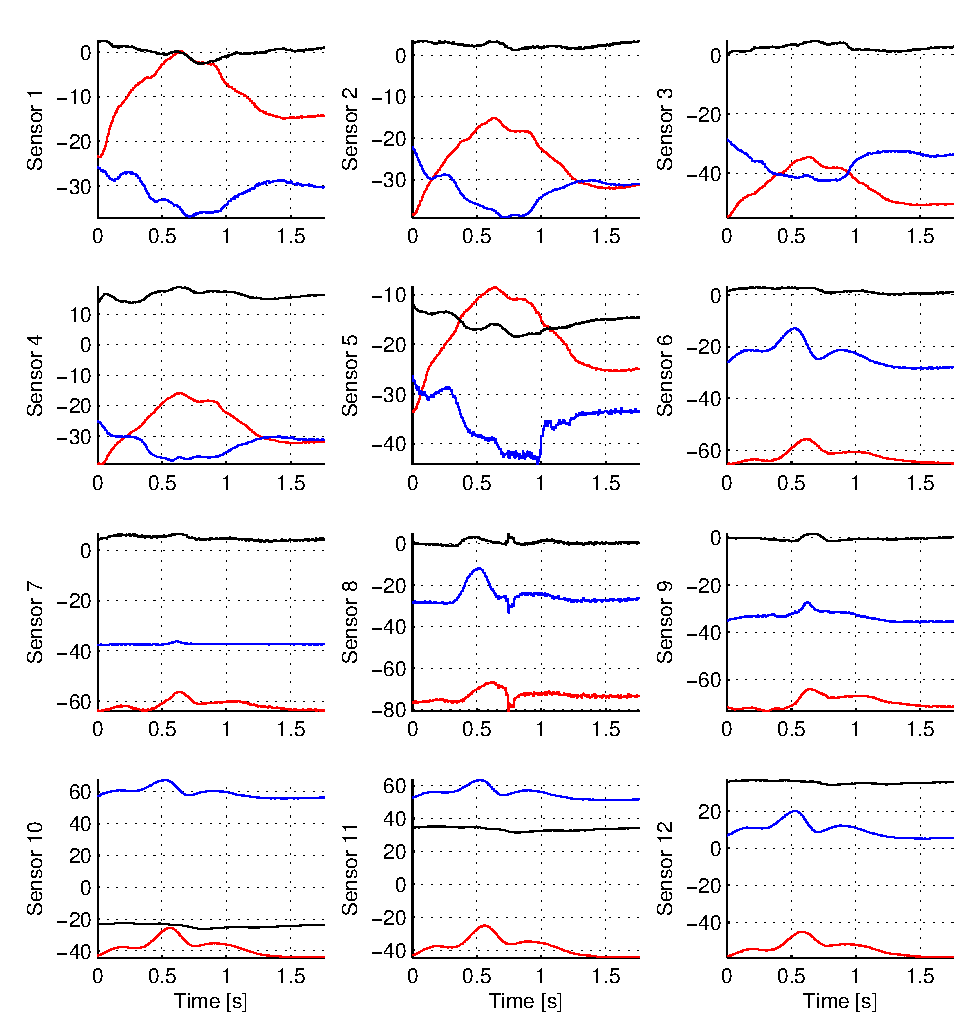
\includegraphics[width=0.45\textwidth]{include/results/images/final_15_trj.eps}}
	\hspace{0.05\textwidth}
	\subfigure[\label{fig:results:giallo:trj}]
	{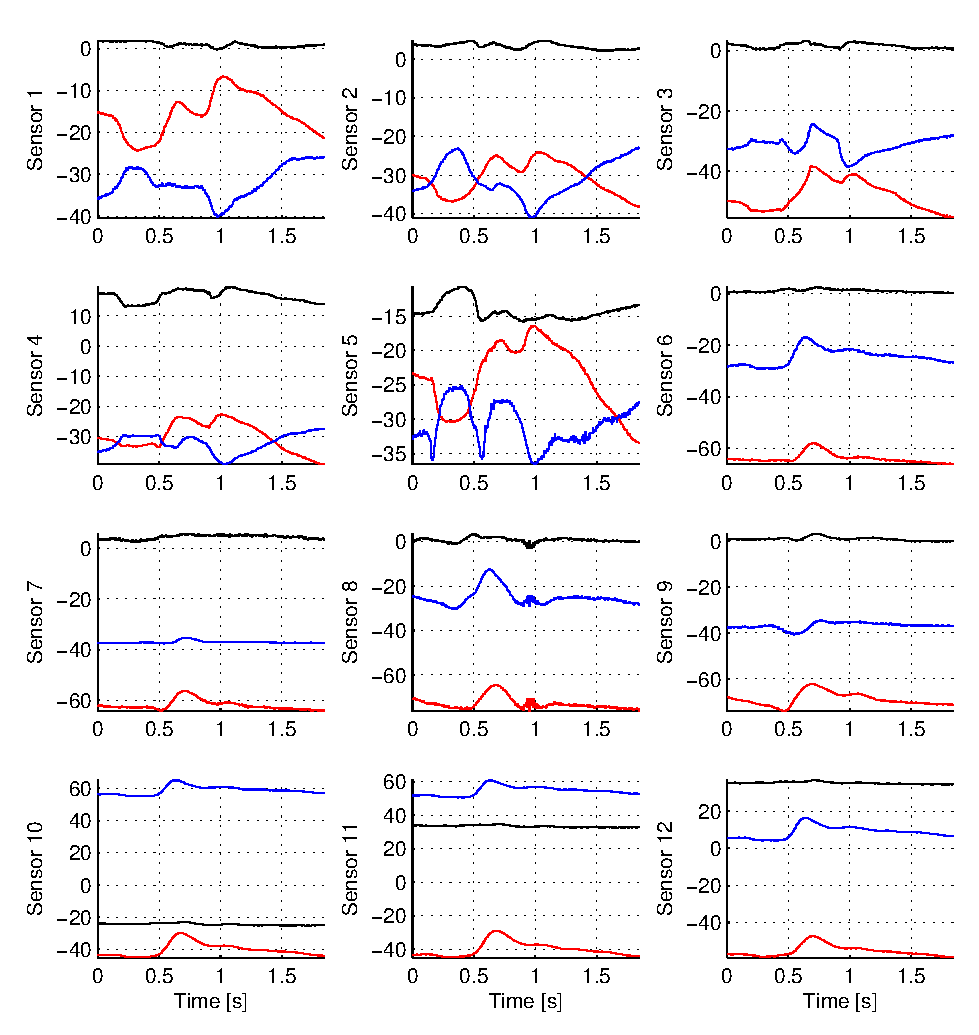
\includegraphics[width=0.45\textwidth]{include/results/images/final_20_trj.eps}}
%	\hspace{0.05\textwidth}

	\caption[Trajectories of the sensors for /uovo/ and /giallo/]{\textbf{Trajectories
	of the sensors for /uovo/ and /giallo/}: the trajectories of the twelve
	sensors during the pronunciation of the words  (a) /uovo/ and
	(b) giallo are here shown.
	The red curves represent the \emph{x} Cartesian component of the
	trajectories, while the black and the blue ones represent the \emph{y} and 
	\emph{z} coordinates.
	Note: the \emph{Phi} and \emph{Theta} angles are not shown.}
	\label{fig:results:trajectories}
\end{figure}
% ---------------------------------------------------------------------------- %
